\documentclass{sig-alternate-05-2015}
\usepackage[utf8]{inputenc} %Umlaute
\usepackage{graphicx}

\makeatletter
\def\@copyrightspace{\relax}
\makeatother

\begin{document}

\title{Convolutional Neural Networks for Image Classification}

\numberofauthors{1}
\author{
\alignauthor
Laura Anger\\
       \affaddr{Institute for Media and Imaging Technology}\\
       \affaddr{TH K\"oln -- University of Applied Sciences Cologne}\\
       \email{laura.anger@smail.th-koeln.de}
}
      
\maketitle
\begin{abstract}
This paper shows the structure and functionality of both - normal NN and CNN. By showing the disatvantages of NNs when it comes to image classification and processing it shows the power of CNNs. 
\end{abstract}

\keywords{Convolutional Neural Networks ; Image Classification}

\section{Introduction}

The Localisation and Recognition of the human visual system is very efficient, even when it has to deal with cluttered scenes. But this is not a matter of course for machines. And also image classification is important in many different areas, the algorithms are not at its best. To show the diversity of approaches, here is a list of typical application: traffic sign recognition \cite{6033458}\cite{6033589}, face recognition, or even detection of  content, which should not be seen by minors \cite{7545022}. Image classification is also a part of medicine, as there are approaches which can detect small cells. It is obvious that there are many more fields, which could be mentioned here. \\\\
For machines it is still a difficult challenge, because real-world images differ regarding various characteristics as discribed detailed in \cite{6033589} and completed in \cite{ijcai2011}.
Due to Neural Networks (NN), Image Classification becomes more and more fast and stabil (Quote??). There are examples, where the automatic classification is better than the human visual system \cite{6033458}. 
In the Literature the NN by Kunihiko Fukushima, which is called Neocognitron is often mentioned and known as the first one of its kind. It is an hierarchical multi-layered artificial neural network, which is used, for example, in the recognition of hand-written characters and in other pattern recognition tasks \cite{Fukushima1980}. It can be seen as an inspiration for many recent variants \cite{ijcai2011}.\\
This paper gives a brief overview of the functionality of NNs and describes how they can be trained using backpropagation. It will also deal with the problems NNs have, when it comes to image processing or especially image classification. Afterwards CNNs are introduced. By comparing the Networks the additional benefit of CNNs is shown. In chapter different approaches of imageclassification using CNNs are presented and discussed. 
\\


1) Bildklassifizierung ist in sehr vielen Bereichen wichtig: pornographische Inhalte filtern, google suche, Straßenschild erkennung, Gesichtserkennung, medizinische Erkennung von Zellen. 

2) Schwierigkeit bei realen Bildern: difficult challenges due to real-world variabilities such as viewpoint variations, lighting condi- tions (saturations, low-contrast), motion-blur, occlusions, sun glare, physical damage, colors fading, graffiti, stickers and an input resolution as low as 15x15 (\cite{6033589} in Introduction )

3) Bildklassifizierung kann unter umständen besser als durch Menschen geschehen (\cite{6033458} im Abstract)

4) Paperaufteilung: erst NN und dann CNN um Vorteile zu verdeutlichen; Anschließend Ansätze schildern
GLIEDERUNG DES PAPERS:
- Einführung in die Thematik und Benennung der Problematik von normalen nn
- Was ist besser an cnn und kurze Funktionsweise
- Cnn paper müssen sortiert dargestellt werden


ÜBERSICHT ENTWICKLUNG NEURONALE NETZE: 
- Neocognitron von Kunihiko Fukushima (1980): hierarchisches mehrschichtiges künstliches neuronales Netz, welches zum Beispiel bei der Erkennung handschriftlicher Zeichen und bei anderen Mustererkennungs-Aufgaben zum Einsatz kommt ( \cite{Fukushima1980} )


\section{Neural Networks}
\subsection{Structure} \label{NNstructure}
There is no general structure of a NN. There are only a few different models and approaches. A NN generally consists of different elements, structures and rules. But to understand the funciotnality of a NN it is important to get an idea of the structure. The following explanations refer to the modell-structure in picture \ref{bildfehlt}\\
A NN has at least to layers. This is why people often refer to it as a Multilayer-Perceptron (MLP).\\

- Eingangsschicht: verteilt nur\\
- 1. Verdeckte Schicht: erzeugt Linien\\
- 2. Verdeckte Schicht: erzeugt Fläche (Polygone ohne Löcher)\\
- Ausgangsschicht: erzeugt beliebige Flächen (konvex, konkav, mit Löchern, beliebig)\\

- BILD AUFBAU NN \\
- Aufbau eines Neurons (auch vergleichen mit Mensch)\\

After understanding the structure of a NN. One can easliy point out the anaolgie to the human NN, which is often mentioned. In both systems the neutrons have multiple entrances but only one exit. The sysnapses connect the exits in the human body with the entrances of other neurons. At this point it should be mentioned, that in a NN only the next layer is connected to the one before. This is different when it comes to the human body. What both systems have in common is, that the 	cell nucleus calculates the output signal out of the many input signals. \\
-->4) Analogie von NN zu menschlichem Körper (Viele Eingänge aber nur einen Ausgang; Synapsen verbinden Ausgang mit den Eingängen anderer Neuronen; Zellkern berechnet aus dem Eingangsignal das Ausgangsgnal)

A regular neural network or multi-layer perceptron (MLP) is made up of input/out layers and a series of hidden layers. 





- Multilayer-Perceptron


\subsection{Functionality}
\subsection{Learning/Backpropagation}

BP in 5 Epoches: \cite{ijcai2011}
\subsection{Pros and Cons for Image Processing and Classification}
There are three main problems if we use MLP for image recognition tasks:


MLPs do not scale well
The generalization performance of the MLP will be eclipsed by its excessive free parameters, i.e., weights. For example, each image from the ImageNet  has a size of 256x256x3. That means each neuron in the hidden layer will have 256x256x3=196608 connections with each pixel in the input image. The total number of weights would scale up quickly if we want to add more neurons or hidden layers. The enormous number of weights produced by full connectivity would quickly lead to overfitting.


MLPs ignore pixel correlation
It is an important property of images that nearby pixels are more strongly correlated than distant pixels. This property is not taken advantage of by MLP due to the full connectivity. This property suggests local connectivity is preferred.

MLPs are not robust to image transformations
It is expected that the recognition algorithm should be robust to transformations applied to the input image. For example, for handwritten digit recognition, a particular digit should be assigned the same value regardless of its position within the image or of its size.

For MLPs, any subtle change in scale or position from the input layer would produce significant changes in following layers. It is therefore advantageous to incorporate into the network some invariance to common changes that could occur in images, e.g., translation, scale, etc.

Accordingly image recognition tasks require a new type of neural network: cnn.

Unsupervised learning methods applied to patches of natu- ral images tend to produce localized filters that resemble off- center-on-surround filters, orientation-sensitive bar detectors, Gabor filters. These findings as well as exper- imental studies of the visual cortex justify the use of such filters in the so-called standard model for object recognition, whose filters are fixed, in contrast to those of Convolutional Neural Networks (CNNs), whose weights (filters) are learned in a supervised way through back-propagation (BP).(\cite{6033458} Muss noch feiner zitiert werden)

\section{Convolutional Neural Networks}

To utilize the prior knowledge on image recognition, CNNs incorporate the following concepts into the design:

Local connectivity
Local connectivity is a solution to the over-parameterization problem. The advantage of using local features and the derived high order features has been demonstrated in classical work in visual recognition. This knowledge can be easily built into the network, by forcing the neurons to receive only local information.


Figure 2. A neural network with local connectivity [5]

This notion is illustrated in Fig. 2 where layer m-1 can be considered as input images, and layer m is the hidden layer. It can be seen from the figure that each neuron in the hidden layer connects to only 3 adjacent input pixels in the image. Local connectivity also takes advantage of the pixel correlation from input image, as each neuron in the hidden layer only cares about nearby pixels in a neighborhood.

Weight sharing
One problem of image recognition tasks is that images that contain the same semantic object could have the object at various locations on the image. As a result, classical work in visual recognition detects local features at various location on the input image. Weight sharing is a solution that stimulates the approach of applying local feature detectors at different positions of the image. It is also a solution to improve network robustness against image transformations.


Figure 3. A neural network with weight sharing [5]

As depicted in Figure 3, the three neurons in hidden layer m share the same weight. Weights of the same colour are constrained to be identical. Note that the hidden layer m could contain multiple planes of neurons that share the same weights. These planes are referred to as "feature maps". Neurons in every feature map are constrained to have identical weights, which is equivalent to performing the same operation in different parts of the image.

Since each neuron is only connected to part of an image, and keeps the information in the corresponding feature map. This behavior is equivalent to a convolution with a small size kernel, followed by a squashing function [2]. This is also how CNN was named.

Sub sampling
As an object can appear at various locations on the input image, the precise location of a local feature is not important to the classification. That means the network can afford to lose the exact position information. However an approximate position information should be retained so that the next layer can possibly detect higher- order feature. As a result the feature maps need not be as the same size of the input image. Instead, a feature map can be built by sub sampling the input image. Sub sampling provides a form of invariance to distortions and translations.

Piecing these concepts together results in LeNet, the first CNN, which is illustrated in Fig 4 [5]. Although Fig 4 does not precisely reflect the architecture presented in [2], it can still be used as an meaningful illustration.



\subsection{structure of CNN}
As already mentioned in chapter \ref{NNstructure} CNNs do not have a general structure as well. The model shown in \ref{fig:CNNstructure} is idealist and would be modified to meet the requirements of the given problem or task. \\
In general it can be said, that a CNN consists of four main steps: convolution, subsampling, activation and full connectedness. There is an additional step called loss for training. This also can be seen in the most popular implementation of the CNN, which is called the LeNet, after Yann LeCun (QUELLE).\\
The colvolutional layers, which are marked in \ref{fig:CNNstructure} receive an input signal.

	
https://www.quora.com/What-is-a-convolutional-neural-network	
	
\begin{figure*}
	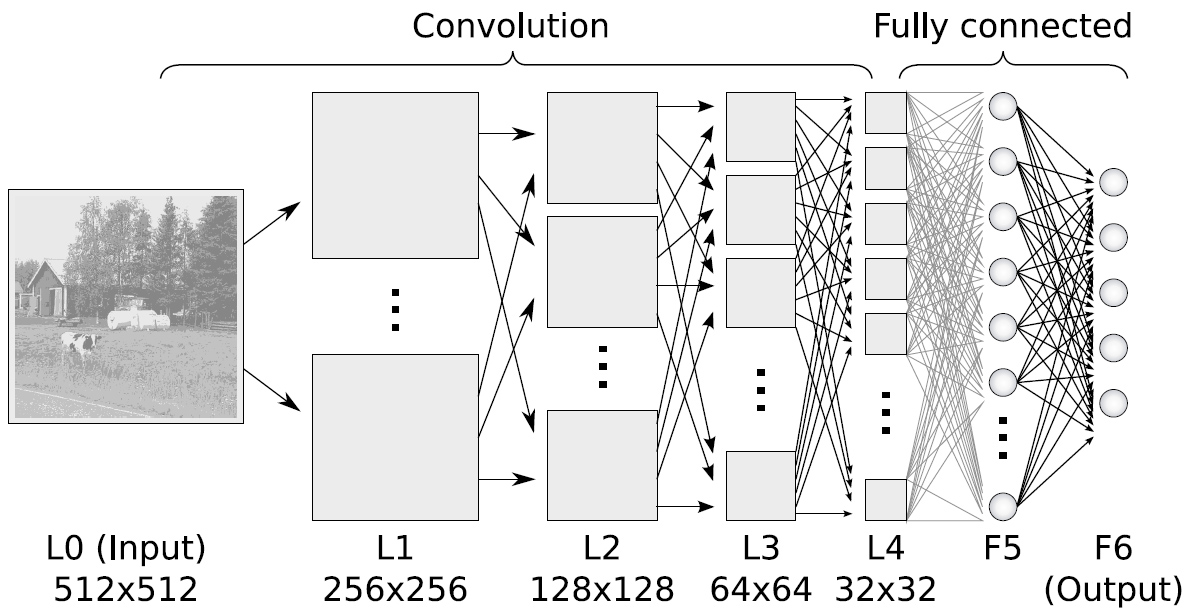
\includegraphics[width=\textwidth]{../Bilder/structure-cnn.jpg}
	\caption{ simple Structure of a CNN \cite{UniBonn}.}
	\label{fig:CNNstructure}
\end{figure*}
	
\subsection{Differences between NN and CNN }
\subsection{pros and cons for image processing/classification }

\subsection{Unterschiede zwischen max-pooling layer und sub-sampling layer??}
max-pooling layer: \cite{6033458}


\section{Different approaches of image classification using CNN}
\section{Conclusion}




\bibliographystyle{abbrv}
\bibliography{cnn} 

\balancecolumns

\end{document}
